% -*- coding: utf-8 -*-
% !TEX encoding = UTF-8 Unicode
% !TEX root =  main.tex

\chapter{Beispiel Kapitel}
\label{chap:beispiel-kapitel}

\section{Abbildungen}\label{sec:abbildungen}

Eine Abbildung lässt sich einfach über:

\lstset{language=TeX}
\begin{lstlisting}
\begin{figure}[htb]
\includegraphics{..pfad/foc-ac-dc.pdf}
\caption{Beschriftung der Abbildung}
\label{fig:foc-ac-dc}
\end{figure}
\end{lstlisting}

einfügen.
Die breite der Abbildung kann einerseits skaliert oder direkt im Maßstab von \SI{14.5}{\centi\meter} erstellt werden.
Wenn die Abbildung maßstabsgetreu erstellt wird, muss \verb|\centering| und der optionale Befehl \verb|[width=\textwidth]| nicht zwingend übernommen werden.

\begin{figure}[htb]
	\centering
	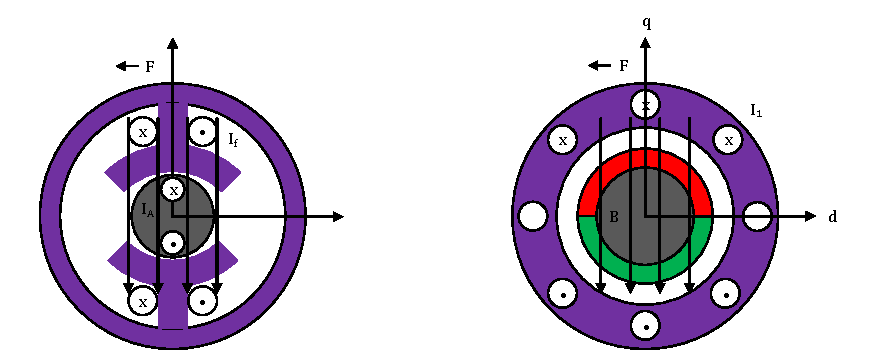
\includegraphics[width=\textwidth]{_images/chapter1/foc-dc-ac.pdf}
	\caption{Beschriftung der Abbildung}
	\label{fig:foc-dc-ac}
\end{figure}

Für Zitationen wird \verb|BibLaTeX| verwendet. Als Backend wird \verb|biber| vom Kompiler verlangt.
Biber ist Open Source und kann im CTAN Repository heruntergeladen werden: \url{https://www.ctan.org/pkg/biber}.

\begin{quote}
\enquote{Bei jeder permanentmagneterregten Synchronmaschine ändern sich die Induktivitäten in abhängigkeit von der Last. In erster Linie sind dafür die Sättigungseffekte, aber auch die Kreuzkopplung verantwortlich.} \autocite[S.~2]{ternes2015}
\end{quote}

Im Text zitierte Werke werden über die Syntax \verb|\textcite[S.~2]{ternes2015}| korrekt zitiert. Beispielsweise: Wie in \textcite[S.~2]{ternes2015} erläutert, sind die Induktivitäten abhängig von der Last \ldots

Der aktuelle Stil des Literaturverzeichnisses und der Zitationen ist \verb|alphabetic|, kann aber auch in Absprache geändert werden, dazu empfiehlt es sich, die \verb|BibLaTeX|-Dokumentation zu konsultieren.

\section{Literaturverwaltungsprogramme}

Die Verwaltung des Lizeraturverzeichnisses stellt bei Abschlussarbeiten eine große Herausforderung dar. Um vermeidbaren Fehlern vorzubeugen empfiehlt sich die Nutzung einer sog.\ Literaturverwaltungssoftware. In den meisten Fällen ist ein direkte Export als \verb|biblatex|-Datei integriert, was das einbinden in die Abschlussarbeit deutlich erleichtert.  

\begin{table}[htb]
	\caption{Einführender Überlick über Literaturverwaltungsprogramme}
	\label{tab:literaturverwaltung}
	\begin{tabularx}{1.0\textwidth}{l l l X}
		\toprule
			Programm & OS & Website & Extras\\
		\midrule
			Zotero & Windows, OS X & \href{https://www.zotero.org}{zotero.org} & FireFox Plugin, ISBN Suchfunktion\\
			Mendeley & Windows, OS X & \href{https://www.mendeley.com/}{mendeley.com} & watchfolder\\
			JabRef	& Windows, OS X & \href{http://jabref.sourceforge.net/}{jabref} & natives bibtex Format \\
		\bottomrule
	\end{tabularx}
\end{table}

\section{Tabellen}\label{sec:tables}

Die folgende Tabelle (s.~Tab.~\ref{tab:tabelle-test}) ist ein Beispiel.

\begin{table}[htb]
		\caption{Tabellenüberschrift}
		\label{tab:tabelle-test}
		\centering
	\begin{tabularx}{0.4\textwidth}{l c c}
			\toprule
			Messsung	&	Spannung		&	Strom	\\
			&	\si{\volt}	&	\si{\ampere} \\
			\midrule
			1			&	12.2			&	1.2	\\
			2			&	13.1			&	1.21 \\
			\bottomrule
	\end{tabularx}
\end{table}



\section{Abschließende Hinweise zum anfertigen von wissenschaftlichen Qualifikationsarbeiten}\label{sec:hinweise-wiss-arbeiten}

 Um die Leserlichkeit eines Textes zu verbessern sollten einige typografische Regeln beachtet werden. Eine einführende Lektüre hierfür ist: \fullcite{bier_typokurz_2009}. Bevor Sie sich mit dieser Vorlage auseinadersetzen, sollten Sie dieses Werk gelesen haben.
 
 Für die Einführung in das wissenschaftliche arbeiten mit \LaTeX\ empfehle ich folgendes Buch: \fullcite{schlosser_wissenschaftliche_2014}. Dieses Buch dient lediglich als Einführung und dient dem besseren Verständnis und Umgang mit \LaTeX.
 
 Als \enquote{Standardwerk} für das wissenschaftliche Arbeiten empfehle ich: \fullcite{theisen_wissenschaftliches_2013}.

Das folgende Buch: \fullcite{kornmeier_wissenschaftlich_2013}, ist eine Art \enquote{Kochbuch} für das wissenschaftliche Arbeiten und versucht dieses auch zu vermitteln. Für eine differenzierte Betrachtung empfehle ich die Auseinandersetzung mit anderer Fachliteratur in diesem Bereich.

%%% Local Variables: 
%%% mode: latex
%%% TeX-master: "main.tex"
%%% TeX-open-quote: "\\enquote{"
%%% TeX-close-quote: "}"
%%% LaTeX-csquotes-open-quote: "\\enquote{"
%%% LaTeX-csquotes-close-quote: "}"
%%% End: 
